\documentclass[9pt,serif]{beamer} 
%\usepackage[T1]{fontenc} % Needed for Type1 Concrete
%\usepackage{concrete} % Loads Concrete + Euler VM
\usepackage{amsthm, amssymb, graphicx, tikz, bm, setspace, subfig, grffile, pseudocode, graphics, hyperref,float}
\usepackage{algorithm}
\usepackage[noend]{algpseudocode}
\usepackage{shortcuts,beamerstuff}



\begin{document}

\title {\bfseries{\sc Mapping Gaussian Process priors to\\ Bayesian Neural Networks }}
\author{Daniel Flam-Shepherd, James Requeima and David Duvenaud}
\institute{
\sc{NIPS Workshop on Bayesian Deep Learning} }
\date{ }

\begin{frame}
\titlepage
\end{frame}

%---------------------------------------------------------------------------%
\begin{frame}
\frametitle{The main objective }

Minimize the KL divergence of prior $\pgp (\bm f ) \equiv \mathcal {G} \mathcal {P} (\bm f  | \bm 0, \B K )$ to prior $\pbnn (\bm f |  \bm \phi ) $ 
in function space! Note $\bm \phi$ are variational parameters of $ q(\B w | \bm \phi)$
\begin{align}
    \mathcal K (\bm \phi)&= 
    \kl [\pbnn (\bm f |  \bm \phi ) \mid   \pgp (\bm f )] \\
    &= -\entropy [\pbnn (\bm f |  \bm \phi ) ] 
       - \E_{\pbnn (\bm f |  \bm \phi ) } [\log \pgp (\bm f  ) ]    
\end{align}

But this is infinite! Approximate it by taking expectations over $p(\X)$ :
$$ \elbo _\X (\bm \phi) \equiv \E _{\X \sim p(\X)} [ \mathcal K (\bm \phi) ] $$  
Assume normality of $\pbnn (\bm f |  \bm \phi )$ and use MC estimation:  
\begin{align}
     \elbo _\X (\bm \phi) \approx
  -\half \log |\bm \Sigma _{\bm f}| -
  \frac{1}{S} \sum_{s=1}^S \E _{\X \sim p(\X)} [\log \pgp (\bm f ^{(s)}(\X) ) ]
\end{align}

Now find $ \bm \phi ^* =  \amin{\bm \phi}  \elbo _\X (\bm \phi ) $ 


\end{frame}

%---------------------------------------------------------------------------%


\begin{frame}
\frametitle{Two Experiments with different kernels}

Red are samples of $\pbnn (\bm f (\X) |  \bm \phi^* )$ (optimized ones)! Green are samples from the GP prior and Blue are non-optimized samples of $\pbnn (\bm f (\X) )$.

\begin{figure}[h]\centering
{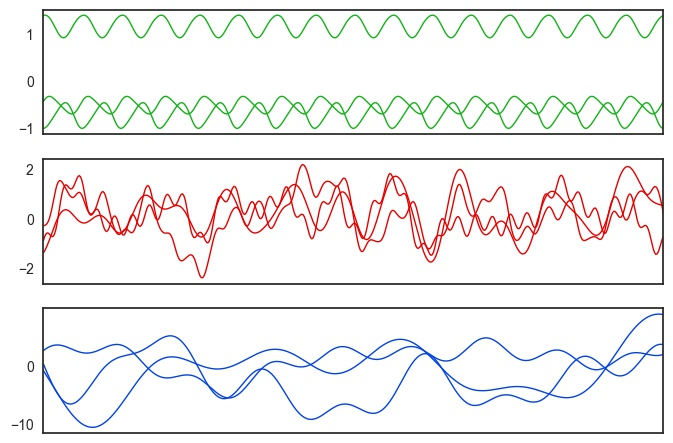
\includegraphics[width=.48\textwidth]{figs/persin2}}
{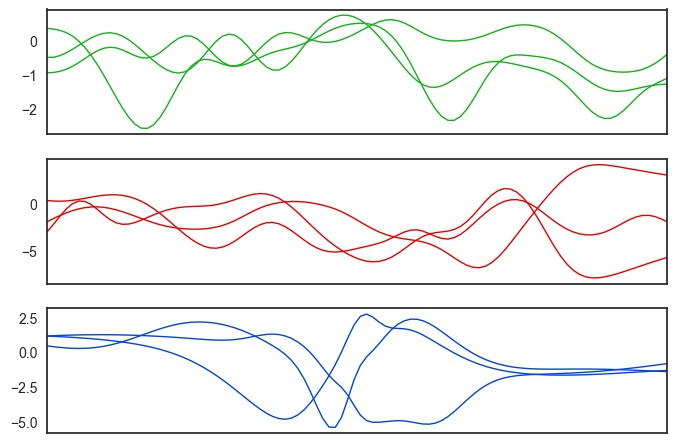
\includegraphics[width=.48\textwidth]{figs/rbfrbf}}
\subfloat[]
{$k(x,x') = e^{-2\sin^2 (\pi| x-x'|) /25 } $}
\hspace{1.5cm}
\subfloat[]
{$k(x,x') = e^{- (x-x')^2/2 }$}
\end{figure}

\centering
Check out our poster!!

\end{frame}

\end{document}

